\documentclass[a4paper, 12pt]{article}
\usepackage{graphicx}
\usepackage{fancyhdr}

\pagestyle{fancy}
\lhead{TDDC78 Lab 5}
\rhead{Hallberg, Svensk}

\begin{document}

\title{TDDC78 Lab 5\\
        Tools }
\author{Christopher Hallberg \\
        Gustav Svensk}
\maketitle

\thispagestyle{empty}

\newpage
\setcounter{page}{1}
\tableofcontents
\newpage

\section{TotalView}
We only used TotalView once in lab 4 to detect an error causing the program to
crash. Before we tried TotalView we used print statements to try to locate the
error but we could not find it. With TotalView we could see at what line the
program crashed and which process caused the crash. It has a good user interface
but since it has so many features and settings it can be difficult to find the
correct ones. When we tried to use more than one node with TotalView is tried to
connect to the other nodes but never succeeded to do so.

We were unable to reproduce the error after fixing it so we do not have any
screenshots.

If we compare TotalView to gdb it is easier to get an overview with TotalView
due to the graphical interface. It is a bit tricky to get gdb to work with
multiple processes whereas TotalView is built for that.

\section{ITAC}
There were some problems using ITAC with full trace where the disc quota on Triolith
was exceeded when using more than a couple of hundred particles. We therefore
ran ITAC twice, one time for the annotated source code with full trace and a
second time with only the MPI tracing functionality. The full trace ran on
four processors with 500 particles each for 30 time steps. The second run without
full tracing used nine processors with 10 000 particles each for 40 time steps.

\subsection{Full Trace}
In the full trace the simulation loop of lab 4 was split into three parts,
collision detection and handling, wall and border crossings and communication. 
Figures \ref{fig:ftt} and \ref{fig:ftsc} shows the event timeline and state
chart. Nothing much can be seen because of the AUTO\_FLUSH, which probably is
connected to all the warnings we received when running full trace. What we can
see is that the only part of the loop that takes up enough time to even show up
on the pie charts is the collision detection and handling. The MPI parts on the
processes (except on the root) are larger because in the last time step they wait for
AUTO\_FLUSH to finish. 

\begin{figure}[h]
        \centering
        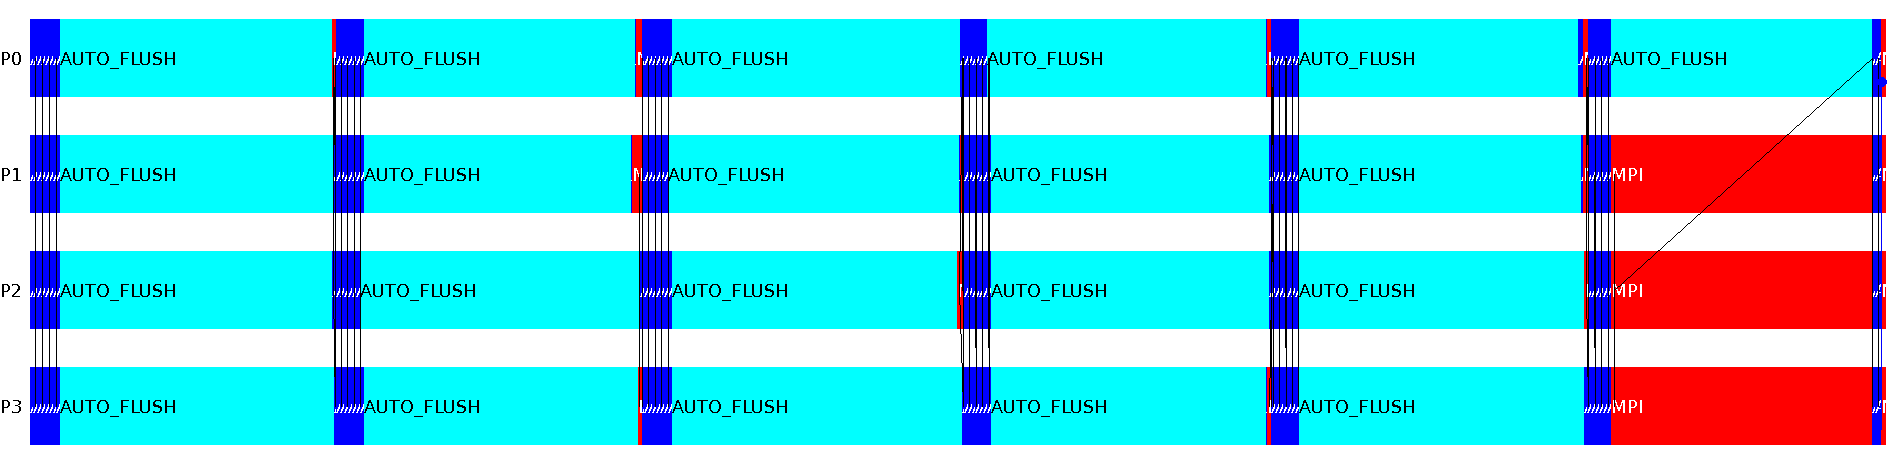
\includegraphics[width=\textwidth]{event_timeline_loop_state.png}
        \caption{Full Trace Timeline}
        \label{fig:ftt}
\end{figure}

\begin{figure}[h]
        \centering
        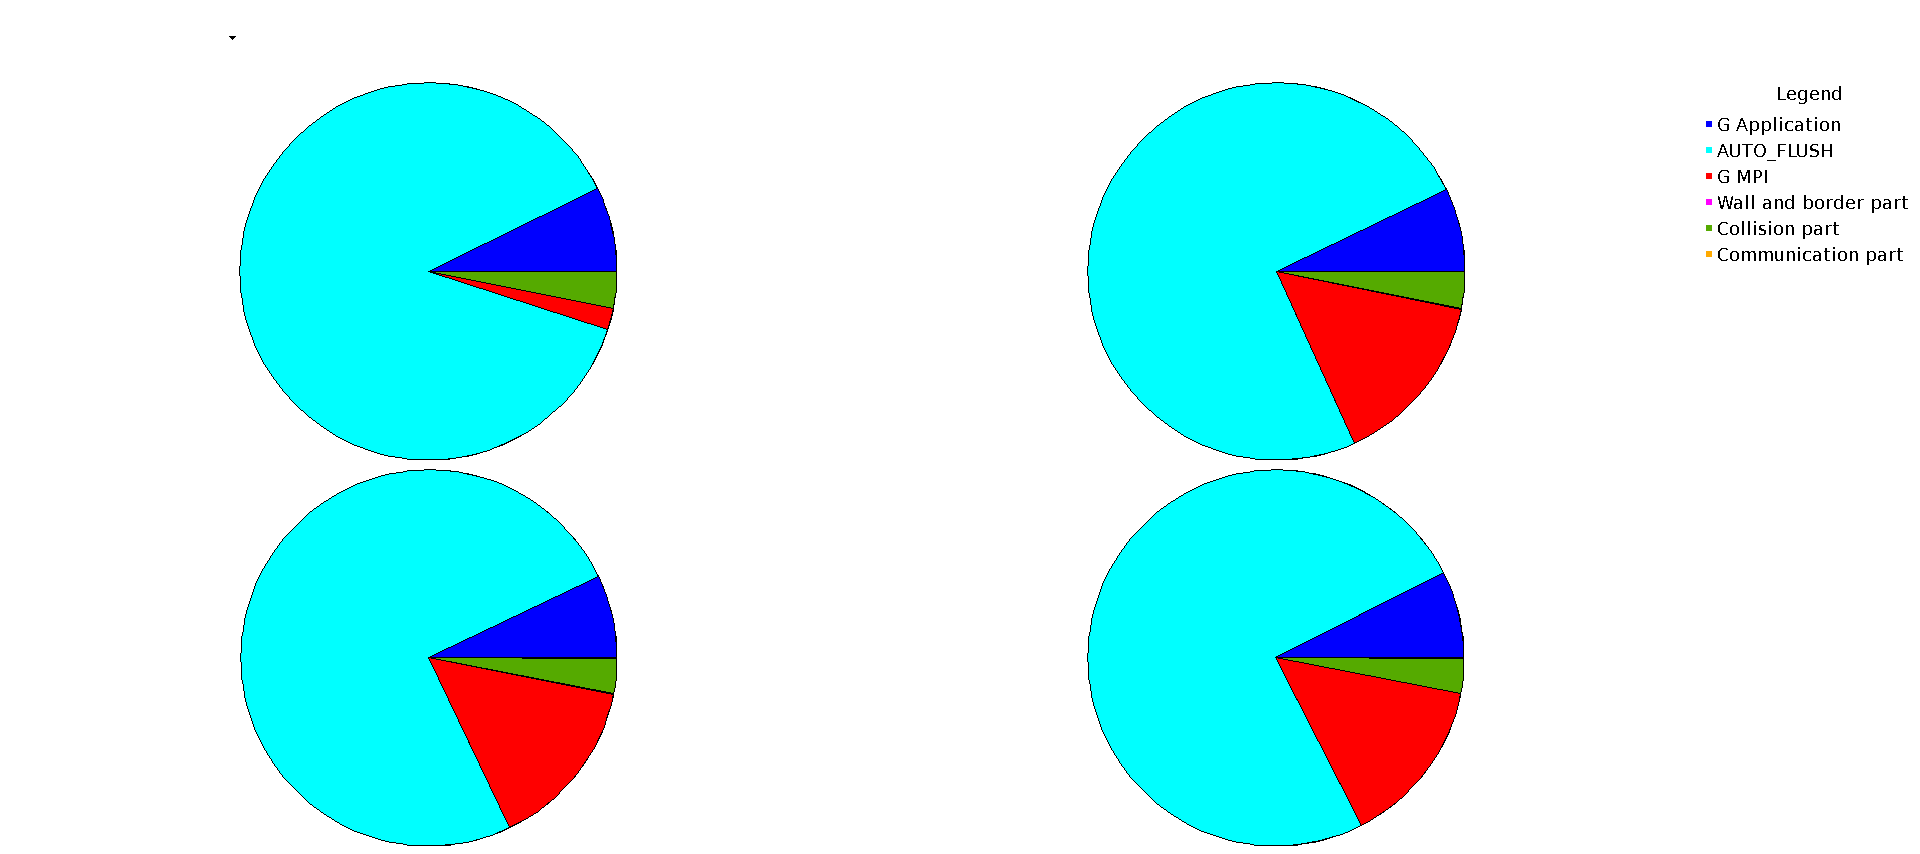
\includegraphics[width=\textwidth]{loop_state_chart.png}
        \caption{Full Trace State Chart}
        \label{fig:ftsc}
\end{figure}
\end{document}
